\documentclass[12pt,a4paper,english]{article}
\usepackage{graphicx}
\topmargin -0.6in
\oddsidemargin=0.0in
\evensidemargin=0.0in
\marginparwidth=0.6in
\textwidth=6.6in
\textheight=9.8in
\begin{document}
	\begin{flushleft}
		Date: 21st May, 2016
	\end{flushleft}
	\begin{center}
		\huge{Sanket R. Bhimani}	
	\end{center}
	\hline
	\begin{flushleft}
		53,Gopal Nagar, \hspace{2.57in}Contact: +919409506643\\
		Near Ambavadi,	\hspace{2.57in}Email-ID: snk.bhimani.jnd@gmail.com\\
		Joshipura,\\
		Junagadh - 362002,\\
		Gujarat.
	\end{flushleft}
	\vspace{-0.6in}
	\begin{figure}[h]
		\begin{flushright}
			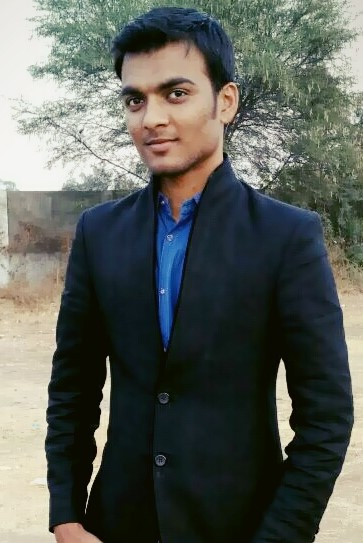
\includegraphics[width=120px]{sanket.jpg}
		\end{flushright}
	\end{figure}
	\hline
	\begin{flushleft}
		\begin{Large}
			\textbf{Objective:}
		\end{Large}\\
		\vspace{0.12in}
		\hspace{0.72in}I am always eager to learn new things whether it's releted with my subject or not.\\
		\vspace{0.3in}
		\begin{Large}
			\textbf{Education:}
		\end{Large}\\
		\vspace{0.12in}
		\hspace{0.72in}
		\begin{tabular}{|c|c|c|c|c|}
			\hline
			Degree&School&University&Year Of Degree&Result Of Degree\\
			 \hline
			 B.tech.&Noble High School,&Dharmsingh Desai University,&2014-2018&CPI: 7.79\\
			 &Junagadh&Nadiad&&&
			 \hline
		\end{tabular}
	\end{flushleft}
\end{document}